\documentclass[10pt]{article}
\usepackage{fancyhdr}
\usepackage{amsmath}
\usepackage{graphicx}
\pagestyle{fancy}
\headheight 35pt
\parskip 10pt \parindent 0pt 
\lhead{Classical Mechanics HW 3}
\chead{Andrei Ilyashenko}
\rhead{09-21-2010}
\cfoot{\thepage}

\begin{document}
%%%%%%%%%%%%%%%%%%%%%%%%%%%%%%%%%%%%%%%%%%%%%%%%%%%%%%%%%%%%%%%%%%%%%%%%%%%%%%%%%%%%
\textbf{Chap 4 Ex 23}\\
\begin{figure}[h!]
    \centering
    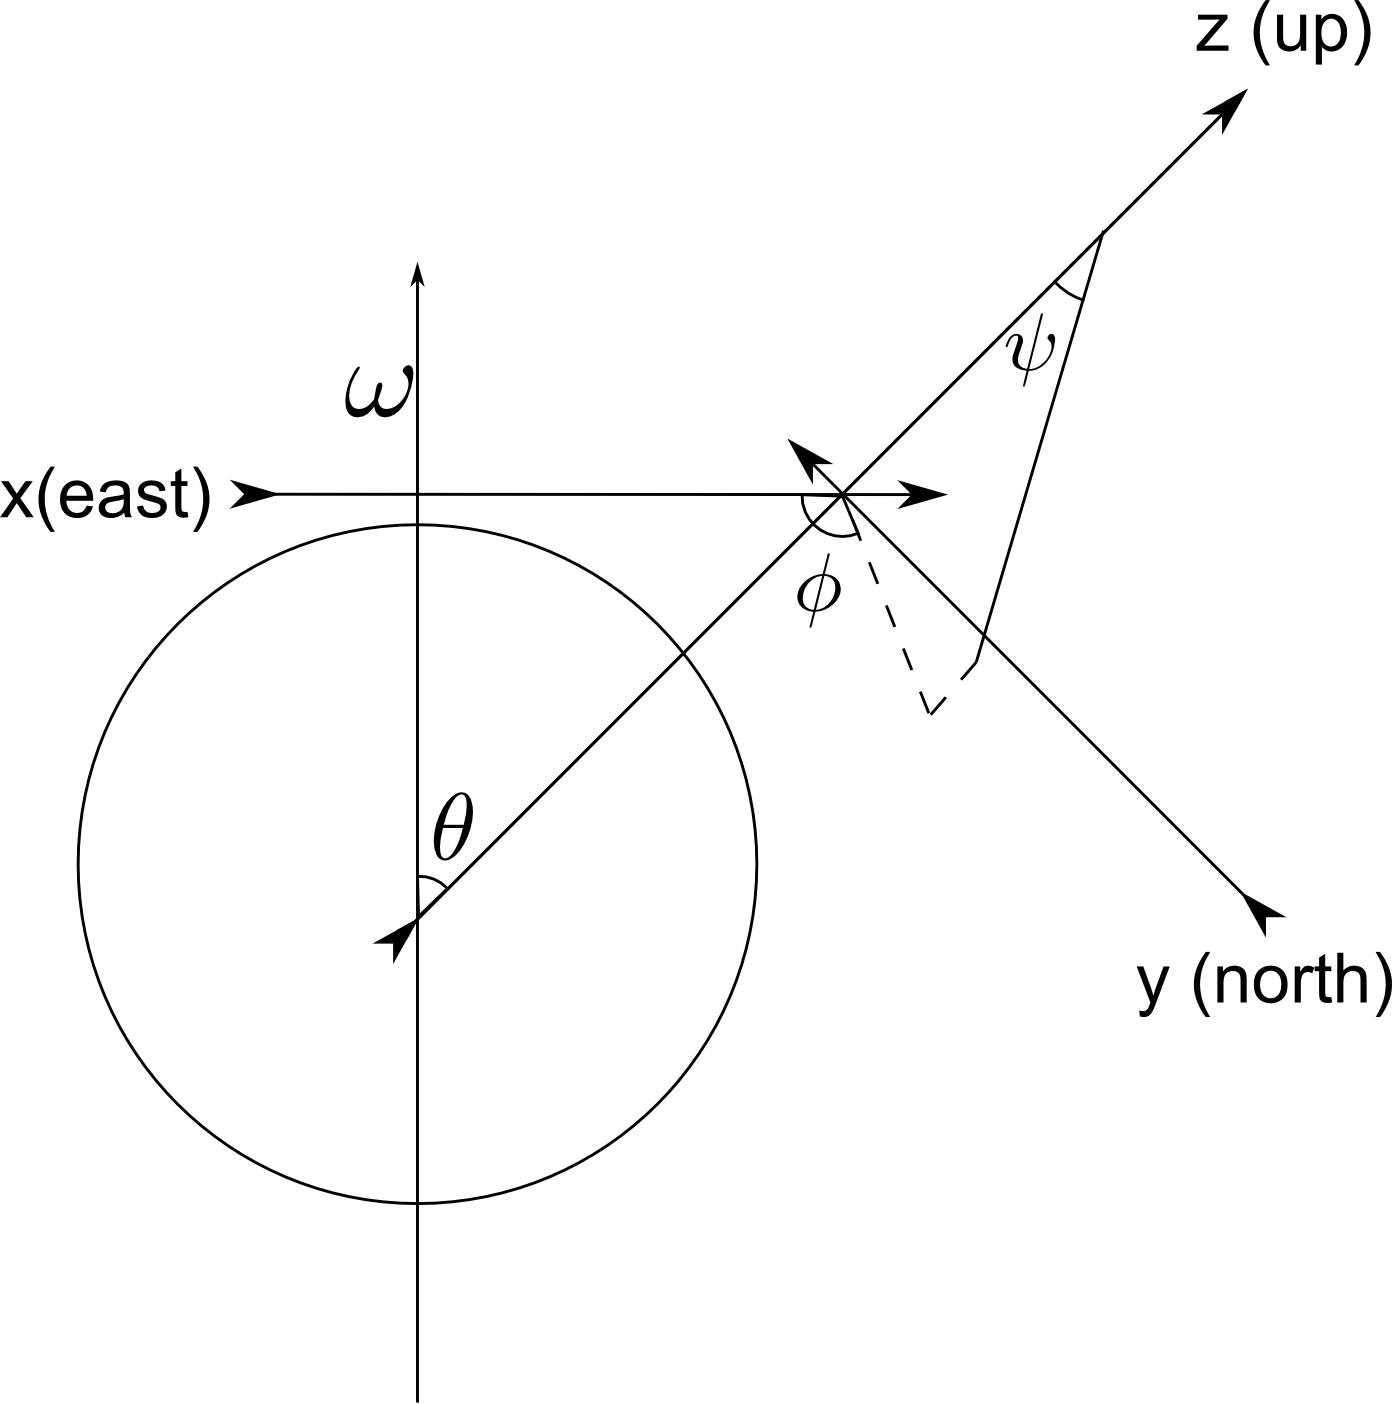
\includegraphics[width=0.7\textwidth]{4Ex23.png}
    \caption{This figure shows the angles used in the Foucault pendulum 
    non-inertial coordinate system.  $\phi$ is the angle between the x axis
    and the projection of the pendulum rod onto the x-y plane.}
  \label{fig:4-23}
\end{figure}
See figure \ref{fig:4-23} for an explanation of the coordinate system.
The equations of motion for the Foucault pendulum in the body frame is
\begin{align*}
  m\ddot r &= \vec T + m\vec g - 2m(\vec\omega\times\dot\vec r).
\end{align*}
The first term is the tension of the string, the second term is the 
acceleration due to gravity (and we can let the centrifugal force be 
absorbed into this term), and the last term is the Coriolis force.
The tension is given by
\begin{align*}
  \vec T &= T(\sin\psi\cos\phi, \sin\psi\sin\phi, \cos\psi),
\end{align*}
and $\vec\omega$ is
\begin{align*}
  \vec\omega &= \omega(-\sin\theta, 0, \cos\theta).
\end{align*}
Thus, $\vec\omega\times\dot\vec r$ is
\begin{align*}
  \vec\omega\times\dot\vec r &= (-\omega\dot y\cos\theta, \omega(t\sin\theta\dot z+\cos\theta\dot x), -\omega\sin\theta\dot y).
\end{align*}
So, for the $\hat z$ direction, the equation of motion is
\begin{align*}
  m\ddot z &= T\cos\psi - mg + 2m\omega\dot y\sin\theta.
\end{align*}
Since the rod or string of the Foucault pendulum is typically very long, and 
only makes a small angle at the top,
it is a good approximation to say that $\ddot z=0$, and $\cos\psi=1$, and
$2m\omega\dot y\sin\theta=0$.  This reduces the equation to
\begin{align*}
  0 &= T - mg\\
  T &= mg.
\end{align*}
Now, we can solve the coupled $x$ and $y$ equations of motion.  They are
\begin{align*}
  \ddot x &= -g\sin\psi\cos\phi + 2\omega\dot y\cos\theta\\
  \ddot y &= -g\sin\psi\sin\phi - 2\omega(\dot x\cos\theta + \dot z\sin\theta).
\end{align*}
Again using the approximation that $\psi$ is very small we can set $\dot z\approx0$, and get
\begin{align*}
  \ddot x &= -g\sin\psi\cos\phi + 2\omega\dot y\cos\theta\\
  \ddot y &= -g\sin\psi\sin\phi - 2\omega\dot x\cos\theta.
\end{align*}
Notice that $l\sin\psi=\sqrt{x^2+y^2}$, $\sqrt{x^2+y^2}\cos\phi = x$, and
$\sqrt{x^2+y^2}\sin\phi = y$, so the two equations above become
\begin{align*}
  \ddot x &= -\frac{g}{l}x + 2\omega\dot y\cos\theta\\
  \ddot y &= -\frac{g}{l}y - 2\omega\dot x\cos\theta.
\end{align*}
If we let $\zeta=x+iy$, and add the above two equations, we get
\begin{align*}
  \ddot \zeta &= -\frac{g}{l}\zeta - i2\omega\cos\theta\dot\zeta\\
  \ddot \zeta + i2\omega\cos\theta\dot\zeta +\frac{g}{l}\zeta &= 0,
\end{align*}
which has the solution 
\begin{align*}
  \zeta(t) &= A e^{i\sigma t},
\end{align*}
where $A$ is a constant determined from the initial conditions, and $\sigma$ is
\begin{align*}
  -\sigma^2-2\sigma\omega\cos\theta+\frac{g}{l} &= 0\\
  \sigma &= \omega\cos\theta\pm\sqrt{\frac{g^2}{l^2}+\omega^2\cos^2\theta}.
\end{align*}
Since $\omega\approx2\pi$ rad per day, we have that the plane of oscillations 
rotates uniformly at a rate of $2\pi\cos\theta$ radians per day.

\textbf{Chap 5 Ex 14}\\
First, we need to calculate the moment of inertia tensor components.  Let the 
z axis pass through the center of the cylinder, and the parallel to its side,
and the the x-y plane cut the cylinder in half and be parallel to the top and
bottom.  Assuming the cylinder has a uniform mass distribution, 
In this coordinate system, the moments of inertia are
\begin{align*}
  I_{zz} &= \int_{\rm{cylinder}}(x^2+y^2)dm\\
  I_{zz} &= \frac{M}{h\pi R^2}\int_{-h/2}^{h/2}\int_{0}^{2\pi}\int_{0}^{R} r^2 rdrd\theta dz\\
  I_{zz} &= \frac{M}{4h\pi R^2}\int_{-h/2}^{h/2}\int_{0}^{2\pi} R^4 d\theta dz\\
  I_{zz} &= \frac{MR^2}{2},
\end{align*}
where $M$ is the mass of the cylinder, and $R$, the radius.  From the symmetry,
the $x$ and $y$ moments of inertia will be the same, and also the off diagonal
terms in the moment of inertia tensor will be 0.  I will calculate, the $x$
component of the moment of inertia, and leave the rest as an exercise
\begin{align*}
  I_{xx} &= \int_{\rm{cylinder}}(z^2+y^2)dm\\
  I_{xx} &= \int_{\rm{cylinder}}(z^2+r^2\sin^2\theta)dm\\
  I_{xx} &= \frac{M}{h\pi R^2}\int_{-h/2}^{h/2}\int_{0}^{2\pi}\int_{0}^{R} (z^2+r^2\sin^2\theta) rdrd\theta dz\\
  I_{xx} &= \frac{M}{h\pi R^2}\int_{-h/2}^{h/2}\int_{0}^{2\pi} \frac{1}{2}\left( z^2R^2+\frac{1}{2}R^4\sin^2\theta \right)d\theta dz\\
  I_{xx} &= \frac{M}{h\pi R^2}\int_{-h/2}^{h/2}\frac{1}{2}\left( 2\pi z^2R^2+\frac{1}{2}\pi R^4 \right) dz\\
  I_{xx} &= \frac{M}{2}\left( \frac{1}{6} h^2+\frac{1}{2} R^2 \right)\\
  I_{xx} &= \frac{M}{12}\left( h^2 + 3R^2 \right).
\end{align*}
The ellipsoid of inertia is given by
\begin{align*}
  I_{xx} x^2 + I_{yy} y^2 + I_{zz} z^2 &= I.
\end{align*}
In order for this to be the equation of a sphere $I_{xx}=I_{yy}=I_{zz}$, so
\begin{align*}
  I_{zz} &= I_{xx}\\
  \frac{MR^2}{2} &= \frac{M}{12}\left( h^2 + 3R^2 \right)\\
  6R^2 &= \left( h^2 + 3R^2 \right)\\
  3R^2 &= h^2\\
  \frac{h}{R} &= \frac{1}{\sqrt 3}\\
  \frac{h}{2\pi R} &= \frac{1}{2\pi\sqrt 3}
\end{align*}
Thus the height to diameter ratio must be $\frac{1}{2\pi\sqrt 3}$ in order for 
the ellipsoid of inertia about the center of the cylinder to be a sphere.
\textbf{Chap 5 Ex 17}\\
\begin{figure}[h!]
    \centering
    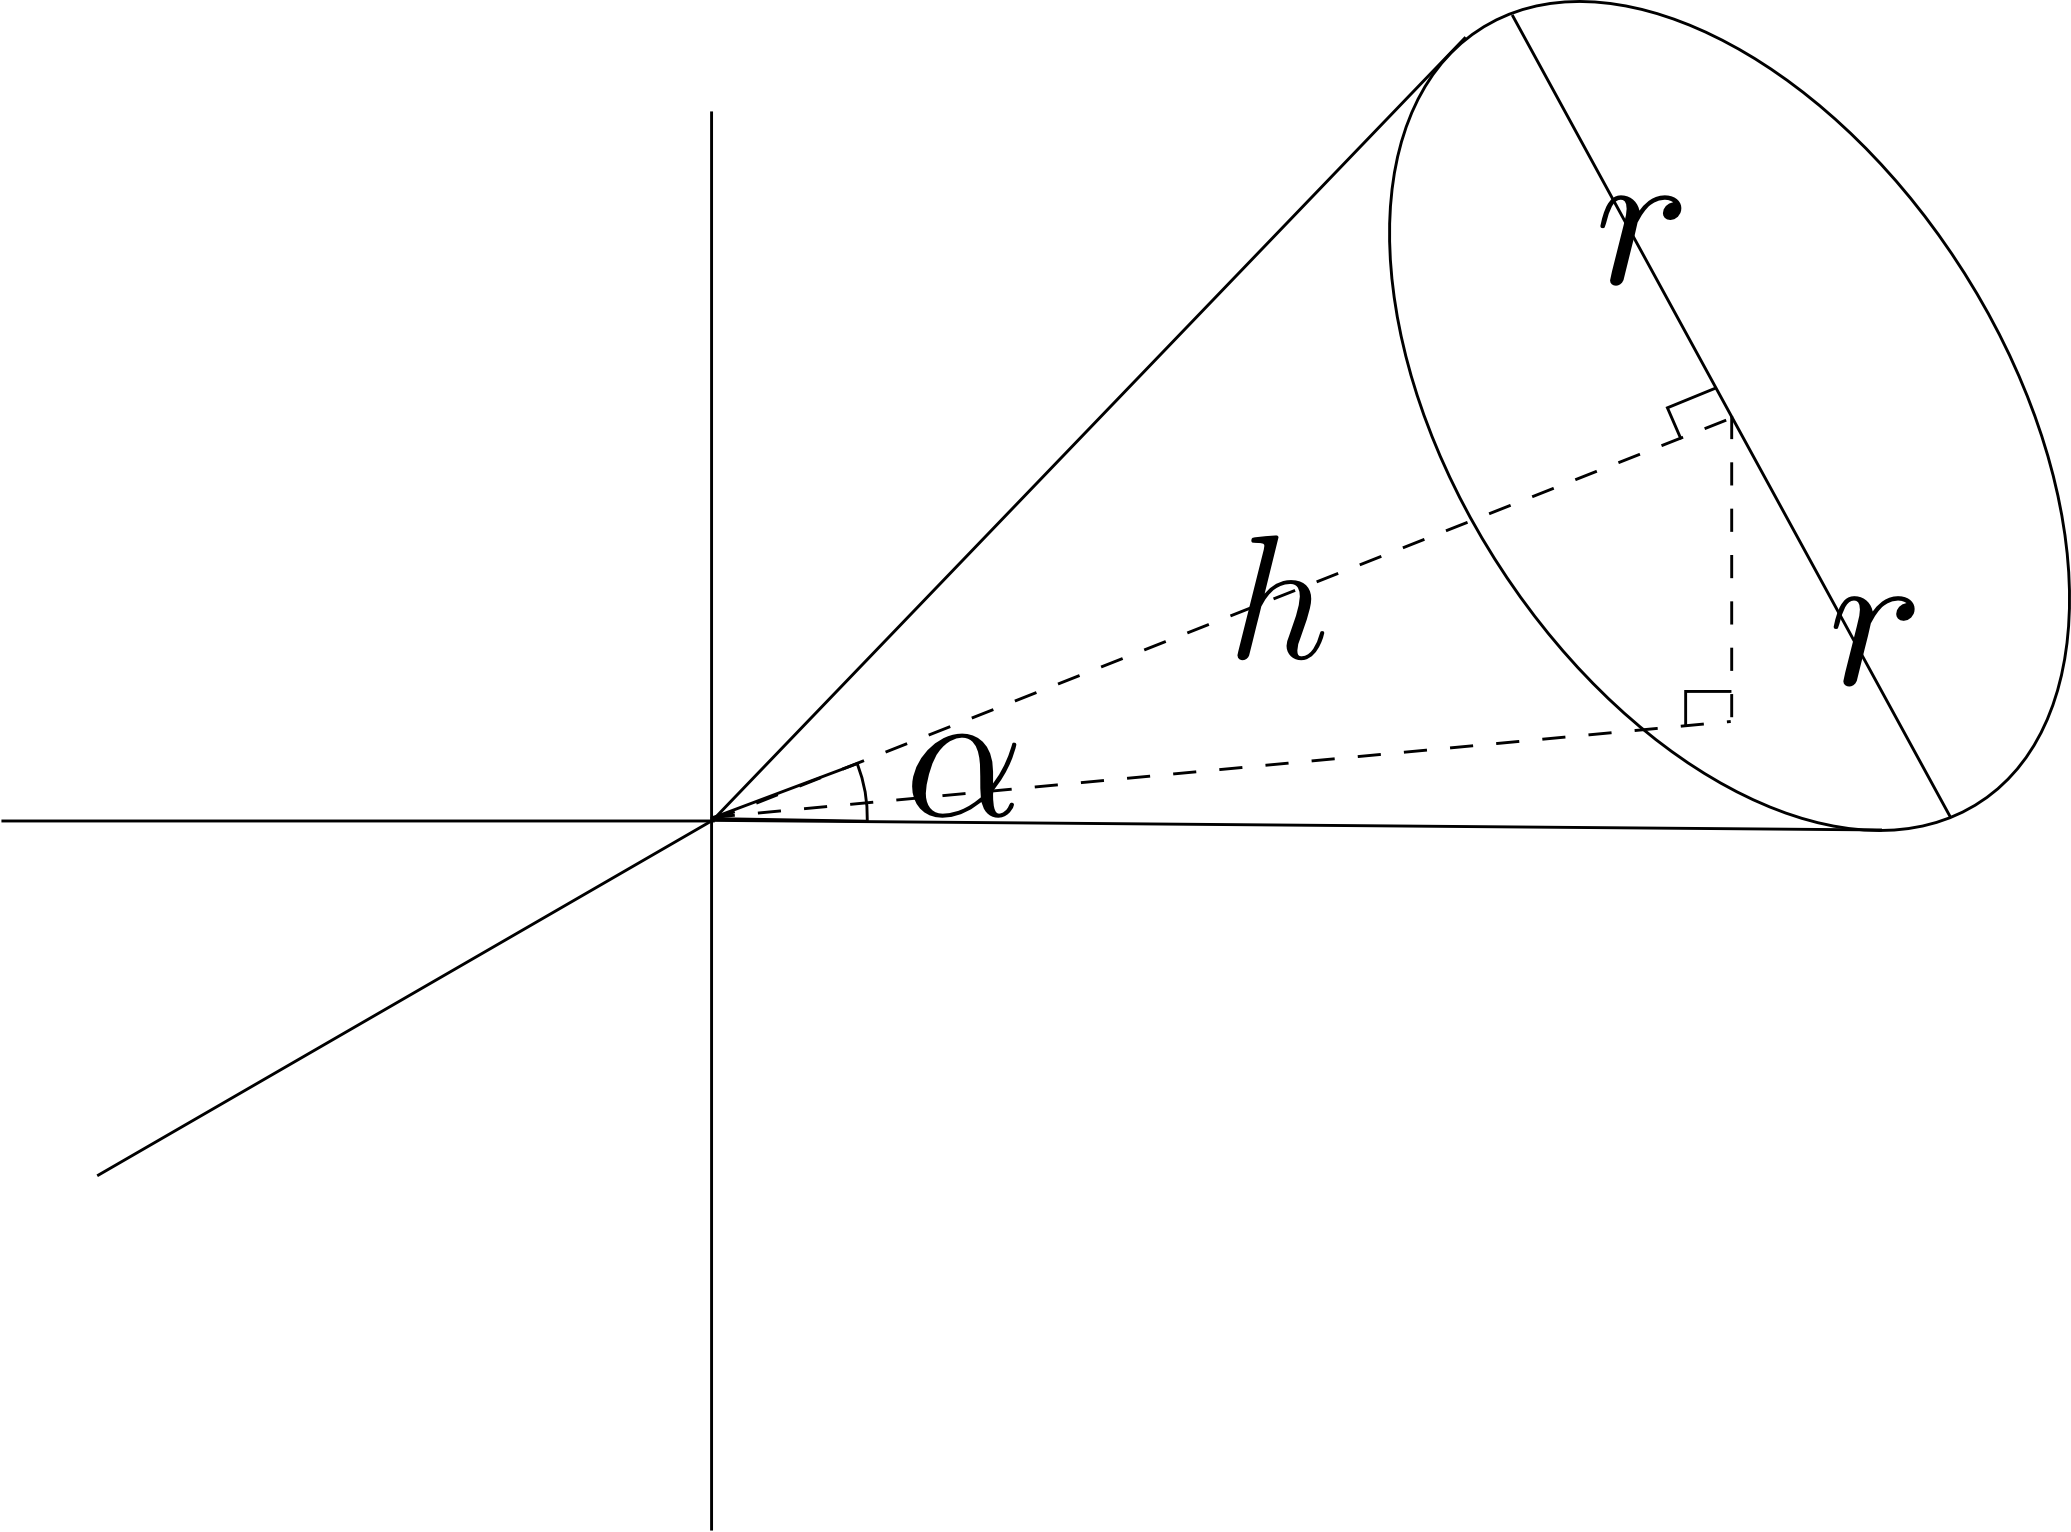
\includegraphics[width=0.7\textwidth]{5Ex17.png}
    \caption{This figure shows the coordinate system for the rolling right
    triangular pyramid.  $r$ is the radius and $\alpha$ is the half angle.}
  \label{fig:5-17}
\end{figure}
See figure \ref{fig:5-17} for an explanation of the coordinate system.
Assuming, that the cylinder rotates with a constant angular velocity, then the
angular momentum is always pointing along the $z$ principal axis, so the 
kinetic energy is
\begin{align*}
  T &= \frac{1}{2}I\omega^2 + T_{\rm{cm}}\\
  T &= \frac{3mr^2}{20}\omega^2 + \frac{1}{2}m(\frac{3h/4}\cos\alpha)^2\frac{4\pi^2}{\tau^2}.
\end{align*}
Where $\omega$, the angular velocity is $\frac{2\pi}{\tau\sin\alpha}$, and the mass is
$m=\rho\frac{1}{3}\pi r^2 h$. So we get
\begin{align*}
  T &= \frac{\rho\pi r^4 h}{20}\frac{4\pi^2}{\tau^2} + \frac{1}{2}m(\frac{3h/4}\cos\alpha)^2\frac{4\pi^2}{\tau^2}\\
  T &= \frac{\rho\pi^3 r^4 h}{5\tau^2\sin^2\alpha} + \frac{6\rho r^2h^3\cos^2\alpha\pi^3}{\tau^2}
\end{align*}
Also substituting $r=h\tan\alpha$ gives
\begin{align*}
  T &= \frac{\rho\pi^3 h^5 \tan^4\alpha}{5\tau^2\sin^2\alpha} + \frac{6\rho h^5\cos^2\alpha\tan^2\alpha\pi^3}{\tau^2}.
\end{align*}
The only terms that have units are $\rho$, which is a density, $h$ which is a
length, and $\tau$ which is a time.  So, both terms have units of mass times
velocity squared, which is energy.
The magnitude of the angular momentum is
\begin{align*}
  L &= I\omega\\
  L &= \frac{2T_{\rm{rotational}}}{\omega}\\
  L &= \frac{\rho\pi^2 h^5 \tan^4\alpha}{5\tau\sin\alpha}.
\end{align*}
and its direction as a function of time is
\begin{align*}
  \hat{L} &= (\cos\alpha\cos\left( \frac{2\pi t}{\tau} \right),\cos\alpha\sin\left( \frac{2\pi t}{\tau}\right),\sin\alpha)
\end{align*}
So, the angular momentum precesses about the z-axis with a fixed magnitude.
\textbf{Chap 5 Ex 22}\\
The length of the rod is $\sqrt{3}r$, so using the parallel axis theorem, 
the moment of inertia for rotation about the center of the circle is
\begin{align*}
  I &= I_{\rm{cm}} + m\frac{r^2}{4}.
\end{align*}
the derivation of the moment of inertia for an infinitely thin rod of mass
$m$ and length $L$ is left as an exercise.
\begin{align*}
  I &= \frac{3mr^2}{12} + m\frac{r^2}{4}\\
  I &= \frac{1}{2}mr^2.
\end{align*}
So, the kinetic energy of the rod is 
\begin{align*}
  T &= \frac{1}{4}mr^2\dot\theta^2.
\end{align*}
Note that there is no translational kinetic energy because the axis of 
rotation (not the center of mass) is fixed.  The potential energy is
\begin{align*}
  V &= -mg\frac{r}{2}\cos\theta.
\end{align*}
So, the Lagrangian is 
\begin{align*}
  L &= T-V\\
  L &= \frac{1}{4}mr^2\dot\theta^2+mg\frac{r}{2}\cos\theta,
\end{align*}
which is equivalent to the Lagrangian of a pendulum of length
$r$ (it is off by a factor of 2, which does not affect the resultant
equations of motion).\\
\textbf{Chap 5 Ex 29}\\
\begin{figure}[h!]
    \centering
    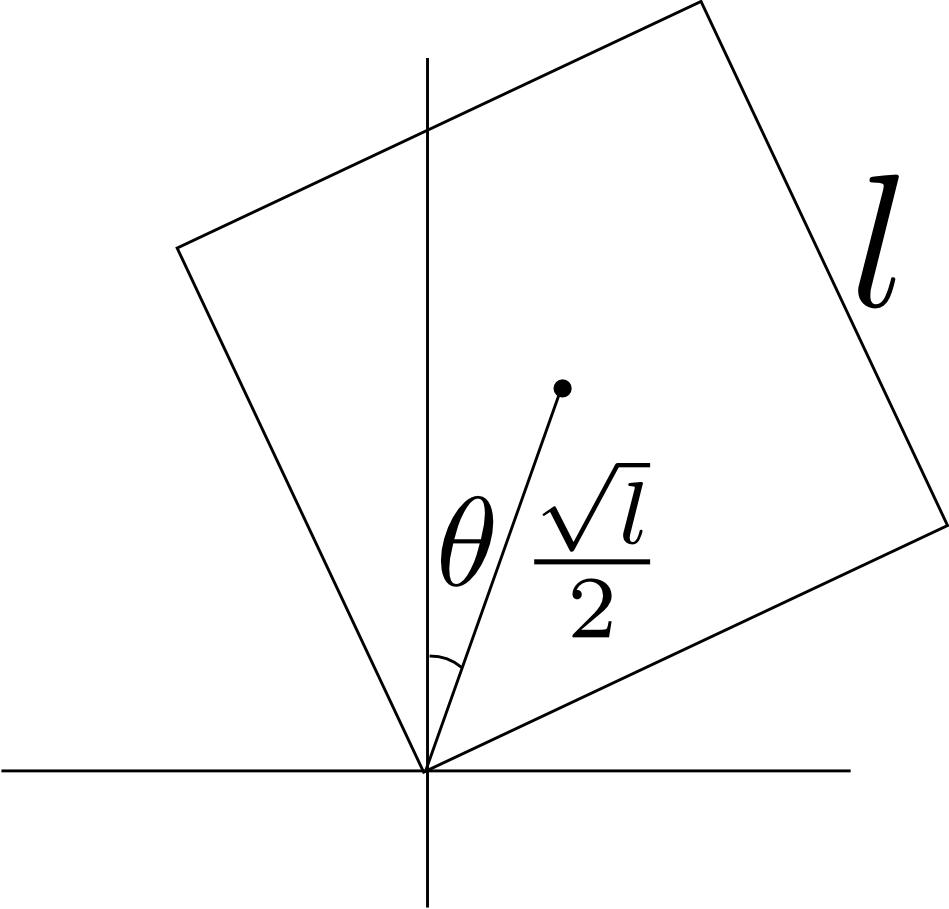
\includegraphics[width=0.7\textwidth]{5Ex29.png}
    \caption{This figure shows the coordinate system for the balanced cube.
    Let $x$ be the location of the edge along the x axis.}
  \label{fig:5-29}
\end{figure}
See figure \ref{fig:5-29} for an explanation of the coordinate system.
Assuming, that the cylinder rotates with a constant angular velocity, then the
If the edge is fixed, then there will be no translational kinetic energy, and
the moment of inertia is 
\begin{align*}
  I &= \frac{ml^2}{6} + \frac{ml^2}{2}\\
  I &= \frac{2ml^2}{3}.
\end{align*}
Again, the simple derivation of the moment of inertia about the center of the 
cube is left as an exercise.  Since there is no translational kinetic energy,
we can use energy conservation to determine the kinetic energy when the 
cube hits the surface, and from that get the angular velocity.  The total 
energy of the system is
\begin{align*}
  E &= T+V = 0+mg\frac{l}{\sqrt{2}}.
\end{align*}
When the cube hits the plane, its gravitational potential energy is
\begin{align*}
  V &= mg\frac{l}{2},
\end{align*}
so, the kinetic energy when it hits the plane is
\begin{align*}
  E &= T+V\\
  mg\frac{l}{\sqrt{2}} &= T + mg\frac{l}{2}\\
  T &= mgl\frac{\sqrt{2}-1}{2}.
\end{align*}
So, the angular velocity is
\begin{align*}
  T &= \frac{1}{2}I\omega^2\\
  mgl\frac{\sqrt{2}-1}{2} &= \frac{ml^2}{3}\omega^2\\
  \omega^2 &= \frac{3g(\sqrt{2}-1)}{2l}\\
  \omega &= \sqrt{\frac{3g(\sqrt{2}-1)}{2l}}.
\end{align*}
If the edge is not fixed, then there will be a translational kinetic energy 
term, but the total kinetic energy will be the same. Also, we will need to 
seperate the kinetic energy into the rotational part (about the center of
mass) and the translational part (of the center of mass).
\begin{align*}
  T &= \frac{1}{2}I\omega^2 + \frac{1}{2}m\left( \left( \frac{l}{\sqrt{2}}\dot\theta\cos\theta+\dot x \right)^2+\frac{l^2}{2}\dot\theta^2\sin^2\theta \right)\\
  T &= \frac{ml^2}{12}\omega^2 + \frac{ml^2}{4}\omega^2 + \frac{1}{2}m\dot x^2 + m\frac{l}{\sqrt{2}}\dot\theta\dot x\cos\theta\\
  T &= \frac{ml^2}{3}\omega^2 + \frac{1}{2}m\dot x^2 + m\frac{l}{\sqrt{2}}\dot\theta\dot x\cos\theta,
\end{align*}
where $x$ is the position of the edge. Notice that if $\dot x=0$ we get the
same result as before.  The potential energy is
\begin{align*}
  V &= mg\frac{l}{\sqrt{2}}\cos\theta.
\end{align*}
So, the Lagrangian equation for $x$ will be.
\begin{align*}
  \frac{d}{dt}\left( m\dot x + \frac{ml}{\sqrt{2}}\dot\theta\cos\theta \right) &= 0\\
\end{align*}
This implies that the quantity $m\dot x + \frac{ml}{\sqrt{2}}\dot\theta\cos\theta$
is conserved.  At time zero, it has a value of 0, therefore
\begin{align*}
  \dot x &= -\frac{l}{\sqrt{2}}\dot\theta\cos\theta,
\end{align*}
and when the cube hits the plane this expression becomes
\begin{align*}
  \dot x &= -\frac{l}{2}\dot\theta.
\end{align*}
This expression matches what intuition would predict, since intuition tells us
that as the cube rotates to the right, its edge will move the the left.
Now, using this equation and conservation of energy we can solve for $\dot x$
and $\dot\theta$,
\begin{align*}
  T &= mgl\frac{\sqrt{2}-1}{2}\\
  \frac{ml^2}{3}\omega^2 + \frac{1}{2}m\dot x^2 + m\frac{l}{\sqrt{2}}\dot\theta\dot x\cos\theta &= mgl\frac{\sqrt{2}-1}{2}\\
  \frac{ml^2}{3}\omega^2 + \frac{ml^2}{8}\omega^2 - m\frac{l^2}{4}\omega^2 &= mgl\frac{\sqrt{2}-1}{2}\\
  \frac{ml^2}{3}\omega^2 + \frac{ml^2}{8}\omega^2 - \frac{ml^2}{4}\omega^2 &= mgl\frac{\sqrt{2}-1}{2}\\
  5ml^2\omega^2 = 12mgl(\sqrt{2}-1)\\
  \omega = \sqrt{\frac{12g(\sqrt{2}-1)}{5l}}.
\end{align*}
Notice that this angular velocity is greater than the angular velocity we get
if the edge is fixed.  This is because the cube is sliding to the left as it
rotates counterclockwise.  This causes the total kinetic energy to decrease, 
and to ensure that energy is conserved, it must rotate faster than it would
if the cube was not sliding.

\end{document}
